\section{How to use OTB?}

\begin{frame}
\frametitle{How to use OTB?}
\vspace{-0.5cm}
\begin{center}
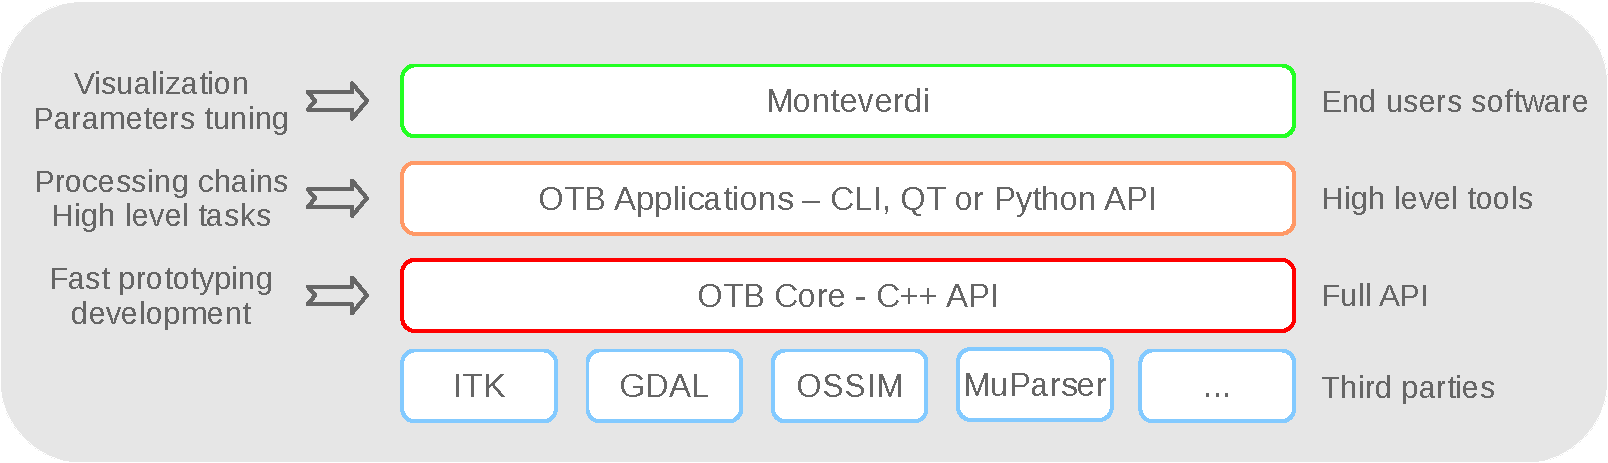
\includegraphics[width=\textwidth]{images/sandwich.pdf}
\end{center}
\vspace{-0.5cm}
\begin{block}{Write your own code}
 Flexible, access to full API, requires C++ knowledge
\end{block}
\begin{block}{Use the applications}
 High level functions (e.g. segmentation), callable from CLI, Qt, Python, can be extended
\end{block}
\begin{block}{Use Monteverdi}
Visualization, data management, \textcolor{red}{Access to all applications}
\end{block}
\end{frame}

\begin{frame}[fragile]
\frametitle{Show me the code!}
\begin{lstlisting}[language=c++,breaklines=true,breakatwhitespace=true,frame = tb,framerule = 0.25pt,fontadjust,backgroundcolor={\color{listlightgray}},basicstyle = {\ttfamily\tiny},keywordstyle = {\ttfamily\color{red}\textbf},identifierstyle = {\ttfamily},commentstyle = {\ttfamily\color{listcomment}\textit},stringstyle = {\ttfamily},showstringspaces = false,showtabs = false,numbers = none,numbersep = 2pt, numberstyle={\ttfamily\color{listnumbers}},tabsize = 2]
#include "otbImage.h"
#include "otbImageFileReader.h"
#include "otbImageFileWriter.h"
#include "itkCannyEdgeDetectionImageFilter.h"
#include "itkRescaleIntensityImageFilter.h"

int main(int argc, char * argv[])
{
  typedef double                      PixelType;
  typedef otb::Image<PixelType>       ImageType;

  typedef unsigned char               OutputPixelType;
  typedef otb::Image<OutputPixelType> OutputImageType;

  typedef otb::ImageFileReader<ImageType> ReaderType;
  ReaderType::Pointer reader = ReaderType::New();

  reader->SetFileName(argv[1]);

  typedef itk::CannyEdgeDetectionImageFilter
  <ImageType, ImageType> FilterType;
  FilterType::Pointer filter = FilterType::New();

  filter->SetInput(reader->GetOutput());

  typedef otb::ImageFileWriter<OutputImageType> WriterType;
  WriterType::Pointer writer = WriterType::New();

  writer->SetFileName(argv[2]);

  writer->SetInput(filter->GetOutput());

  writer->Update();
}
\end{lstlisting}
\end{frame}


\begin{frame}
\frametitle{The applications: write it once, use everywhere}
\begin{columns}
\column{0.5\textwidth}
\begin{itemize}
\item 87 applications are shipped with OTB
\item 1 application $=$ 1 dynamic library (plugin)
\item Applications are auto-descriptive and auto-documented
\item Applications can be extended outside of OTB
\item Several plugins players:
\begin{itemize}
  \item Command-line
  \item Qt auto-generated
  \item Python
\end{itemize}
\item Applications are meant for integration in external systems
\end{itemize}
\column{0.5\textwidth}
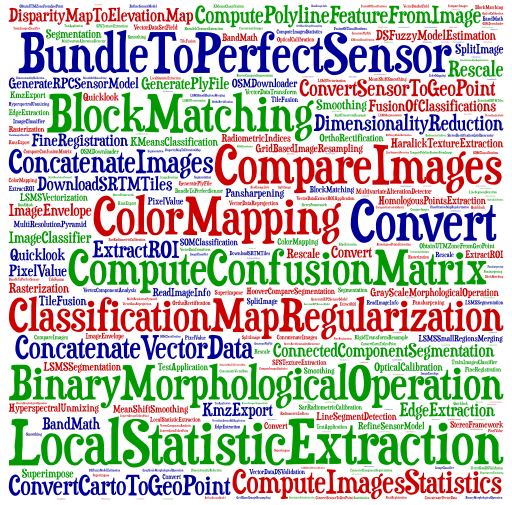
\includegraphics[width=\textwidth]{images/cloud_applications.png}
\end{columns}
\end{frame}



\begin{frame}[fragile]
\frametitle{Applications: command-line invocation}
\begin{scriptsize}
\vspace{-0.5cm}\begin{verbatim}
$ otbcli_OrthoRectification

ERROR: Waiting for at least one parameter...
This is the OrthoRectification application, version 5.2.1
This application allows to ortho-rectify optical images from supported sensors.

Complete documentation: http://www.orfeo-toolbox.org/Applications/OrthoRectification.html

Parameters:
        -progress                <boolean>        Report progress
MISSING -io.in                   <string>         Input Image  (mandatory)
MISSING -io.out                  <string> [pixel] Output Image  [pixel=uint8/uint16/int16/uint32/int32/float/double] (default value is float) (mandatory)
        -map                     <string>         Output Cartographic Map Projection [utm/lambert2/lambert93/wgs/epsg] (mandatory, default value is utm)
        -map.utm.zone            <int32>          Zone number  (mandatory, default value is 31)
        -map.utm.northhem        <boolean>        Northern Hemisphere  (optional, off by default)
        -map.epsg.code           <int32>          EPSG Code  (mandatory, default value is 4326)
        -outputs.mode            <string>         Parameters estimation modes [auto/autosize/autospacing/outputroi/orthofit] (mandatory, default value is auto)
MISSING -outputs.ulx             <float>          Upper Left X  (mandatory)
MISSING -outputs.uly             <float>          Upper Left Y  (mandatory)
MISSING -outputs.sizex           <int32>          Size X  (mandatory)
MISSING -outputs.sizey           <int32>          Size Y  (mandatory)
MISSING -outputs.spacingx        <float>          Pixel Size X  (mandatory)
MISSING -outputs.spacingy        <float>          Pixel Size Y  (mandatory)
        -outputs.lrx             <float>          Lower right X  (optional, off by default)
        -outputs.lry             <float>          Lower right Y  (optional, off by default)
        -outputs.ortho           <string>         Model ortho-image  (optional, off by default)
        -outputs.isotropic       <boolean>        Force isotropic spacing by default  (optional, on by default)
        -outputs.default         <float>          Default pixel value  (optional, on by default, default value is 0)
        -elev.dem                <string>         DEM directory  (optional, off by default)
        -elev.geoid              <string>         Geoid File  (optional, off by default)
        -elev.default            <float>          Default elevation  (mandatory, default value is 0)
        -interpolator            <string>         Interpolation [bco/nn/linear] (mandatory, default value is bco)
\end{verbatim}
\end{scriptsize}
\end{frame}


\begin{frame}[fragile]
\frametitle{Applications: Graphical interface}
\begin{center}
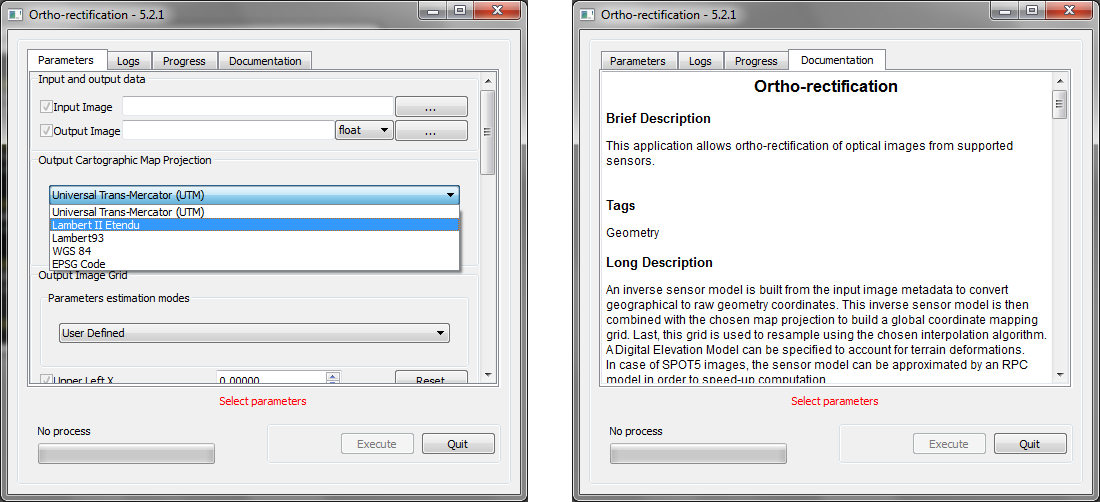
\includegraphics[width=1\textwidth]{images/otbgui.png}
\end{center}
\end{frame}

\begin{frame}[fragile]
\frametitle{Applications: Python interface}
\begin{lstlisting}[language=python,breaklines=true,breakatwhitespace=true,frame = tb,framerule = 0.25pt,fontadjust,backgroundcolor={\color{listlightgray}},basicstyle = {\ttfamily\tiny},keywordstyle = {\ttfamily\color{listkeyword}\textbf},identifierstyle = {\ttfamily},commentstyle = {\ttfamily\color{listcomment}\textit},stringstyle = {\ttfamily},showstringspaces = false,showtabs = false,numbers = none,numbersep = 6pt, numberstyle={\ttfamily\color{listnumbers}},tabsize = 2]
#!/usr/bin/python

# Import the otb applications package
import otbApplication

# The following line creates an instance of the OrthoRectification application
OrthoRectification = otb.Registry.CreateApplication("OrthoRectification")

# The following lines set all the application parameters:
OrthoRectification.IO.IN = "QB_TOULOUSE_MUL_Extract_500_500.tif"
OrthoRectification.IO.OUT = "QB_Toulouse_ortho.tif"

app.MAP = 'epsg'
app.MAP.EPSG.CODE = 32768

# The following line execute the application
OrthoRectification.ExecuteAndWriteOutput()
\end{lstlisting}
\end{frame}


\begin{frame}
\frametitle{Monteverdi (acces to OTB applications)}
\begin{minipage}[t][6cm][t]{\textwidth}
\begin{center}
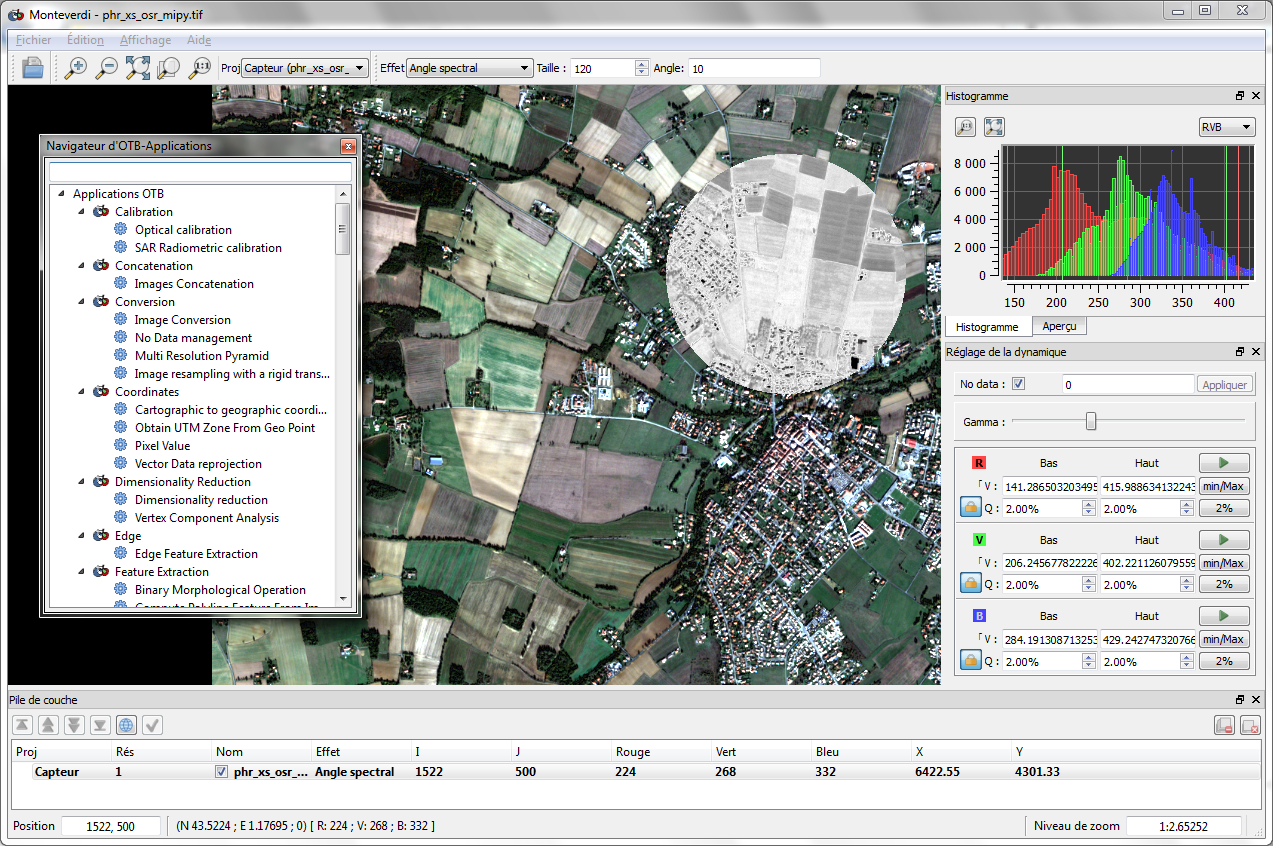
\includegraphics[width=1.0\textwidth]{images/monteverdi.png}
\end{center}
\end{minipage}
\end{frame}

%\vspace*{-3.0mm}
\begin{frame}
  \frametitle{QGIS}
\begin{minipage}[t][6cm][t]{\textwidth}
\begin{center}
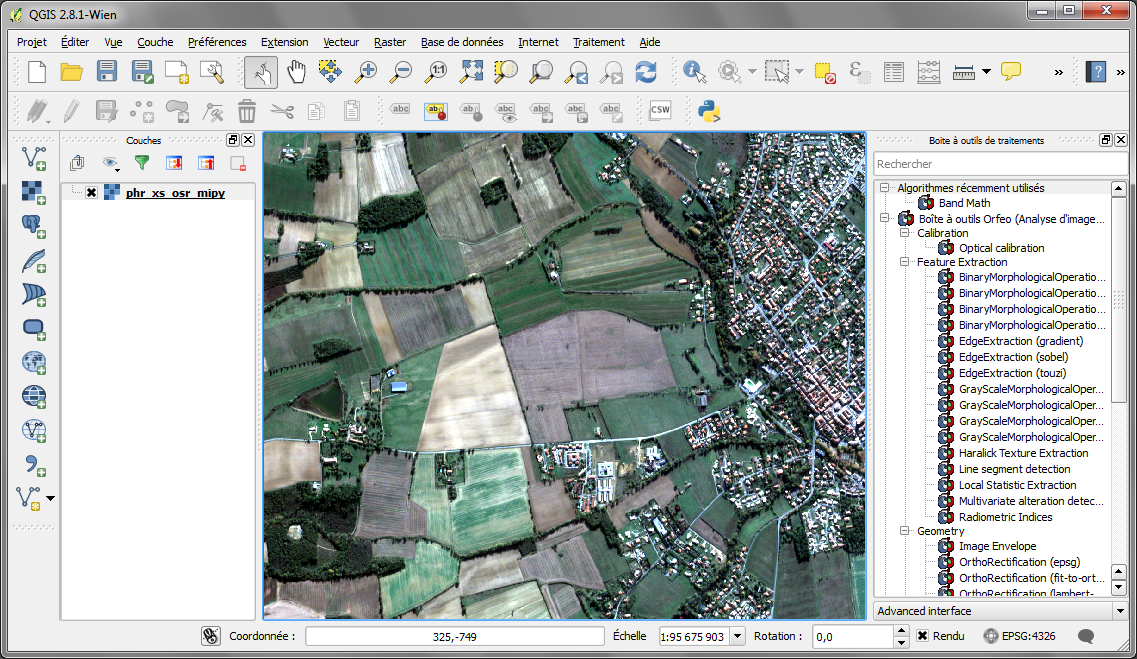
\includegraphics[width=1\textwidth]{images/otb_in_qgis.png}
\end{center}
\end{minipage}
\end{frame}

\begin{frame}
  \frametitle{OTB applications as ZOO WPS service}
\begin{minipage}[t][6cm][t]{\textwidth}
\begin{center}
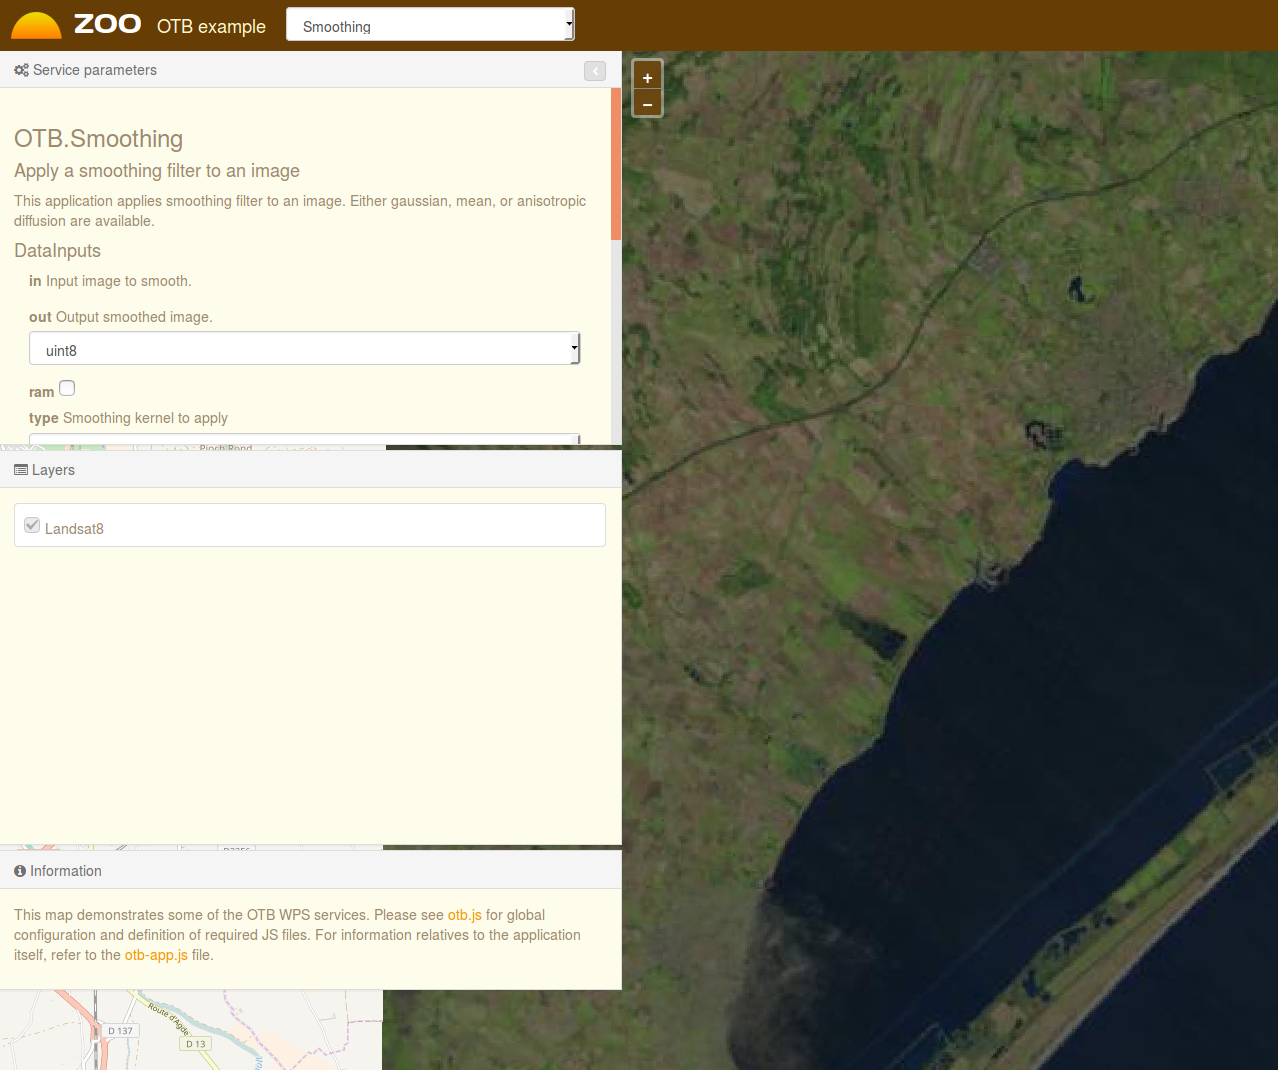
\includegraphics[width=0.7\textwidth]{images/otb_in_zoo.png}
\end{center}
\end{minipage}
\end{frame}
